\documentclass[journal]{IEEEtran}
\usepackage{graphicx}
\usepackage{algorithm}
\usepackage{algpseudocode}
\usepackage{listings}
\usepackage{float}
\usepackage{multirow}

\begin{document}
\section{Instruction Set}
\tiny{
\resizebox{3.5in}{!}{
	\begin{tabular}{|l|l|l|l|l|l|l|}
		\hline
		Instruction Set & Instruction & B & C & Opcode & Operand 1 & Operand 2 \\
		\hline
		\multirow{6}{*}{AND -> A}
		& \texttt{ANL A, Rn} & 1 & 1 & \texttt{01011111} & & \\
		& \texttt{ANL A, direct} & 2 & 1 & \texttt{01010101} & \texttt{<direct>} & \\
		& \texttt{ANL A, @Ri} & 1 & 1 & \texttt{0101011i} & & \\
		& \texttt{ANL A, \#<data>} & 2 & 1 & \texttt{01010100} & \texttt{<data>} & \\
		& \texttt{ANL direct, A} & 2 & 1 & \texttt{01010010} & \texttt{<direct>} & \\
		& \texttt{ANL direct, \#<data>} & 3 & 2 & \texttt{01010011} & \texttt{<direct>} & \texttt{<data>} \\
		\hline
		\multirow{6}{*}{OR -> A}
		& \texttt{ORL A, Rn} & 1 & 1 & \texttt{01001111}  & & \\
		& \texttt{ORL A, direct} & 2 & 1 & \texttt{01000101} & \texttt{<direct>} & \\
		& \texttt{ORL A, @Ri} & 1 & 1 & \texttt{0100011i} & & \\
		& \texttt{ORL A, \#<data>} & 2 & 1 & \texttt{01000100} & \texttt{<data>} & \\
		& \texttt{ORL direct, A} & 2 & 1 & \texttt{01000010} & \texttt{<direct>} & \\
		& \texttt{ORL direct, \#<data>} & 3 & 2 & \texttt{01000011} & \texttt{<direct>} & \texttt{<data>} \\
		\hline
		\multirow{6}{*}{XOR -> A} & \texttt{XRL A, Rn} & 1 & 1 & \texttt{01101nnn}  & & \\
		& \texttt{XRL A, direct} & 2 & 1 & \texttt{01100101} & \texttt{<direct>} & \\
		& \texttt{XRL A, @Ri} & 1 & 1 & \texttt{0110011i} & & \\
		& \texttt{XRL A, \#<data>} & 2 & 1 & \texttt{01100100} & \texttt{<data>} & \\
		& \texttt{XRL direct, A} & 2 & 1 & \texttt{01100010} & \texttt{<direct>} & \\
		& \texttt{XRL direct, \#<data>} & 3 & 2 & \texttt{01100011} & \texttt{<direct>} & \texttt{<data>} \\
		\hline
		rotate ACC right & \texttt{RR A}
		& 1 & 1 & \texttt{00000011} & & \\
		\hline
		rotate ACC left & \texttt{RL A}
		& 1 & 1 & \texttt{00100011} & & \\
		\hline
		rotate ACC right through C
		& \texttt{RRC A} & 1 & 1 & \texttt{00010011} & & \\
		\hline
		rotate ACC left through C
		& \texttt{RLC A} & 1 & 1 & \texttt{00110011} & & \\
		\hline
		swap low and high nibbles in ACC
		& \texttt{SWAP} & 1 & 1 & \texttt{11000100} & & \\
		\hline
		\multirow{2}{*}{set bit low}
		& \texttt{CLR C} & 1 & 1 & \texttt{11000011} & & \\
		& \texttt{CLR <bit>} & 2 & 1 & \texttt{11000010} & \texttt{<bit address>} & \\
		\hline
		\multirow{2}{*}{complement bit}
		& \texttt{CPL C} & 1 & 1 & \texttt{10110011} & & \\
		& \texttt{CPL <bit>} & 2 & 1 & \texttt{10110100} & \texttt{<bit address>} & \\
		\hline
		\multirow{2}{*}{set bit high} &
		\texttt{SETB C} & 1 & 1 & \texttt{11010011} & & \\
		& \texttt{SETB <bit>} & 2 & 1 & \texttt{11010010} & \texttt{<bit address>} & \\
		\hline
		\multirow{4}{*}{single-bit logic}
		& \texttt{ANL C, <bit>} & 2 & 2 & \texttt{10000010} & \texttt{<bit address>} & \\
		& \texttt{ANL C, /<bit>} & 2 & 2 & \texttt{10110000} & \texttt{<bit address>} & \\
		& \texttt{ORL C, <bit>} & 2 & 2 & \texttt{01110010} & \texttt{<bit address>} & \\
		& \texttt{ORL C, /<bit>} & 2 & 2 & \texttt{10100000} & \texttt{<bit address>} & \\
		\hline
		\multirow{2}{*}{bitwise move}
		& \texttt{MOV C, <bit>} & 2 & 1 & \texttt{10100010} & \texttt{<bit address>} & \\
		& \texttt{MOV <bit>, C} & 2 & 2 & \texttt{10010010} & \texttt{<bit address>} & \\
		\hline
		Jump if Carry set
		& \texttt{JC <offset>} & 2 & 2 & \texttt{01000000} & \texttt{<offset>} & \\
		\hline
		Jump if Carry clear
		& \texttt{JNC <offset>} & 2 & 2 & \texttt{01010000} & \texttt{<offset>} & \\
		\hline
		Jump if bit set
		& \texttt{JB <bit>, <offset>} & 3 & 2 & \texttt{00100000} & \texttt{<bit address>} & \texttt{<offset>} \\
		\hline
		Jump if bit clear
		& \texttt{JNB <bit>, <offset>} & 3 & 2 & \texttt{00110000} & \texttt{<bit address>} & \texttt{<offset>} \\
		\hline
		Jump and clear bit if bit set
		& \texttt{JBC <bit>, <offset>} & 3 & 2 & \texttt{00010000} & \texttt{<bit address>} & \texttt{<offset>} \\
		\hline
		\multirow{4}{*}{A + val -> A}
		& \texttt{ADD A, Rn} & 1 & 1 & \texttt{00101nn} & & \\
		& \texttt{ADD A, <direct>} & 2 & 1 & \texttt{00100101} & \texttt{<direct>} & \\
		& \texttt{ADD A, @Ri} & 1 & 1 & \texttt{0010011i} & & \\
		& \texttt{ADD A, \#<data>} & 2 & 1 & \texttt{00100100} & \texttt{<data>} & \\
		\hline
		\multirow{4}{*}{A + val + C -> A}
		& \texttt{ADDC A, Rn} & 1 & 1 & \texttt{00111nnn} & & \\
		& \texttt{ADDC A, <direct>} & 2 & 1 & \texttt{00110101} & \texttt{<direct>} & \\
		& \texttt{ADDC A, @Ri} & 1 & 1 & \texttt{0011011i} & & \\
		& \texttt{ADDC A, \#<data>} & 2 & 1 & \texttt{00110100} & \texttt{<data>} & \\
		\hline
		\multirow{4}{*}{A - val -> A}
		& \texttt{SUBB A, Rn} & 1 & 1 & \texttt{10011nnn} & & \\
		& \texttt{SUBB A, <direct>} & 2 & 1 & \texttt{10010101} & \texttt{<direct>} & \\
		& \texttt{SUBB A, @Ri} & 1 & 1 & \texttt{1001011i} & & \\
		& \texttt{SUBB A, \#<data>} & 2 & 1 & \texttt{10010100} & \texttt{<data>} & \\
		\hline
		\multirow{5}{*}{Increment}
		& \texttt{INC A} & 1 & 1 & \texttt{00000100} & & \\
		& \texttt{INC Rn} & 1 & 1 & \texttt{00001nnn} & & \\
		& \texttt{INC <direct>} & 2 & 1 & \texttt{00000101} & \texttt{<direct>} & \\
		& \texttt{INC @Ri} & 1 & 1 & \texttt{0000011i} & & \\
		& \texttt{INC DPTR} & 1 & 2 & \texttt{10100011} & & \\
		\hline
		\multirow{4}{*}{Decrement}
		& \texttt{DEC A} & 1 & 1 & \texttt{00010100} & & \\
		& \texttt{DEC Rn} & 1 & 1 & \texttt{00011nnn} & & \\
		& \texttt{DEC <direct>} & 2 & 1 & \texttt{00010101} & \texttt{<direct>} & \\
		& \texttt{DEC @Ri} & 1 & 1 & \texttt{0001011i} & & \\
		\hline
		Multiply : low -> A, high -> B
		& \texttt{MUL AB} & 1 & 4 & \texttt{10100100} & & \\
		\hline
		A/B -> A, A\%B -> B
		& \texttt{DIV AB} & 1 & 4 & \texttt{10000100} & & \\
		\hline
		\multirow{16}{*}{dest <- src}
		& \texttt{MOV @Ri, \#<data>} & 2 & 1 & \texttt{0111011i} & \texttt{<data>} & \\
		& \texttt{MOV @Ri, A} & 1 & 1 & \texttt{1111011i} & & \\
		& \texttt{MOV @Ri, <direct>} & 2 & 2 & \texttt{1010011i} & \texttt{<src>} & \\
		& \texttt{MOV A, \#<data>} & 2 & 1 & \texttt{01110100} & \texttt{<data>} & \\ %CHECK
		& \texttt{MOV A, @Ri} & 1 & 1 & \texttt{1110011i} & & \\
		& \texttt{MOV A, <direct>} & 2 & 1 & \texttt{11100101} & \texttt{<src>} & \\
		& \texttt{MOV A, Rn} & 1 & 1 & \texttt{11101nnn} & & \\
		& \texttt{MOV <direct>, <direct>} & 3 & 2 & \texttt{10000101} & \texttt{<dest>} & \texttt{<src>} \\
		& \texttt{MOV <direct>, \#<data>} & 3 & 2 & \texttt{01110101} & \texttt{<dest>} & \texttt{<data>} \\
		& \texttt{MOV <direct>, @Ri} & 2 & 2 & \texttt{1000011i} & \texttt{<dest>} & \\
		& \texttt{MOV <direct>, A} & 2 & 1 & \texttt{11110101} & \texttt{<dest>} & \\
		& \texttt{MOV <direct>, Rn} & 2 & 2 & \texttt{10001nnn} & \texttt{<dest>} & \\
		& \texttt{MOV DPTR, \#<data>} & 3 & 2 & \texttt{10010000} & \texttt{<data|high>} & \texttt{<data|low>} \\
		& \texttt{MOV Rn, \#<data>} & 2 & 1 & \texttt{01111nnn} & \texttt{<data>} & \\
		& \texttt{MOV Rn, A} & 1 & 1 & \texttt{11111nnn} & & \\
		& \texttt{MOV Rn, <direct>} & 2 & 2 & \texttt{10101nnn} & \texttt{<src>} & \\
		\hline
		\multirow{2}{*}{no fucking clue}
		& \texttt{MOVC A, @A+DPTR} & 1 & 2 & \texttt{10010011} & & \\
		& \texttt{MOVC A, @A+PC} & 1 & 2 & \texttt{10000011} & & \\
		\hline
		\multirow{3}{*}{ACC <-> ext. memory}
		& \texttt{MOVX @Ri, A} & 1 & 2 & \texttt{1111001i} & & \\
		& \texttt{MOVX A, @DPTR} & 1 & 2 & \texttt{11100000} & & \\
		& \texttt{MOVX A, @Ri} & 1 & 2 & \texttt{1110001i} & & \\
		\hline
		\multirow{2}{*}{stack operations}
		& \texttt{PUSH <direct>} & 2 & 2 & \texttt{11000000} & \texttt{<src>} & \\
		& \texttt{POP <direct>} & 2 & 2 & \texttt{11010000} & \texttt{<dest>} & \\
		\hline
		\multirow{3}{*}{exchange A and src}
		& \texttt{XCH A, @Ri} & 1 & 1 & \texttt{1100011i} & & \\
		& \texttt{XCH A, <direct>} & 2 & 1 & \texttt{11000101} & \texttt{<src>} & \\
		& \texttt{XCH A, Rn} & 1 & 1 & \texttt{11001nnn} & & \\
		\hline
		exchange low nibble
		& \texttt{XCHD A, @Ri} & 1 & 1 & \texttt{1101011i} & & \\
		\hline
		\multirow{4}{*}{calling subroutines}
		& \texttt{ACALL <direct(11b)>} & 2 & 2 & \texttt{aaa10001} & \texttt{<addr|low>} & \\
		& \texttt{LCALL <direct(16b)>} & 3 & 2 & \texttt{00010010} & \texttt{<addr|high>} & \texttt{<addr|low>} \\
		& \texttt{RET} & 1 & 2 & \texttt{00100010} & & \\
		& \texttt{RETI} & 1 & 2 & \texttt{00110010} & & \\
		\hline
		\multirow{12}{*}{jumping and branching}
		& \texttt{AJMP <direct(11b)>} & 2 & 2 & \texttt{aaa00001} & \texttt{<addr|low>} & \\
		& \texttt{LJMP <direct(16b)>} & 3 & 2 & \texttt{00000010} & \texttt{<addr|high>} & \texttt{<addr|low>} \\
		& \texttt{SJMP <offset(8b)>} & 2 & 2 & \texttt{10000000} & \texttt{<offset>} & \\
		& \texttt{JMP @A+DPTR} & 1 & 2 & \texttt{01110011} & & \\
		& \texttt{JZ <offset(8b)>} & 2 & 2 & \texttt{01100000} & \texttt{<offset>} & \\
		& \texttt{JNZ <offset(8b)>} & 2 & 2 & \texttt{01110000} & \texttt{<offset>} & \\
		& \texttt{CJNE @Ri, \#<data>, <offset(8b)>} & 3 & 2 & \texttt{1011011i} & \texttt{<data>} & \texttt{<offset>} \\
		& \texttt{CJNE A, \#<data>, <offset(8b)} & 3 & 2 & \texttt{10110100} & \texttt{<data>} & \texttt{<offset>} \\
		& \texttt{CJNE A, <direct>, <offset(8b)} & 3 & 2 & \texttt{10110101} & \texttt{<src>} & \texttt{<offset>} \\
		& \texttt{CJNE Rn, \#<data>, <offset(8b)} & 3 & 2 & \texttt{10111nnn} & \texttt{<data>} & \texttt{<offset>} \\
		& \texttt{DJNZ <direct>, <offset(8b)>} & 3 & 2 & \texttt{11010101} & \texttt{<src>} & \texttt{<offset>} \\
		& \texttt{DJNZ Rn, <offset(8b)>} & 2 & 2 & \texttt{11011nnn} & \texttt{<offset>} & \\
		\hline
		do nothing
		& \texttt{NOP} & 1 & 1 & \texttt{00000000} & & \\
		\hline
	\end{tabular}
} %end resizebox


\section{8051 Organization}
Programs can be in either "absolute form", or "relocatable form".
If they are in relocatable form,
linking is required to set the absolute addresses for exocution.

\resizebox{3.5in}{!}{
	\begin{tabular}{r|l}
		ROM & 4K \\
		RAM & 128B \\
		Address Bus & 16b \\
		I/O & 4x 8b parallel ports, 1x serial port (all bit-addressable) \\
	\end{tabular}
} %end resizebox
\begin{center}
	\begin{tabular}{c r|l}
		PSW.7 & \texttt{CY} & 0xD7 \\
		PSW.6 & \texttt{AC} & 0xD6 \\
		PSW.5 & \texttt{F0} & 0xD5 \\
		PSW.4 & \texttt{RS1} & 0xD4\\
		PSW.3 & \texttt{RS0} & 0xD3\\
		PSW.2 & \texttt{OV} & 0xD2\\
		PSW.1 & & 0xD1\\
		PSW.0 & \texttt{P} & 0xD0\\
	\end{tabular}
\end{center}

\subsection{Components}
\resizebox{3.5in}{!}{
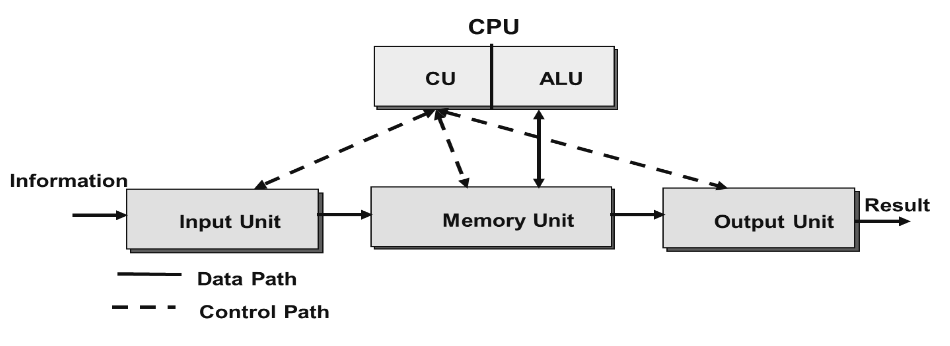
\includegraphics{img/org.png}
}

\subsubsection{Embedded System Advantages}
\begin{itemize}
	\item low power consumption
	\item small size
	\item rugged operating ranges
	\item low unit cost
\end{itemize}


\subsection{Memory Organization}
\resizebox{3.5in}{!}{
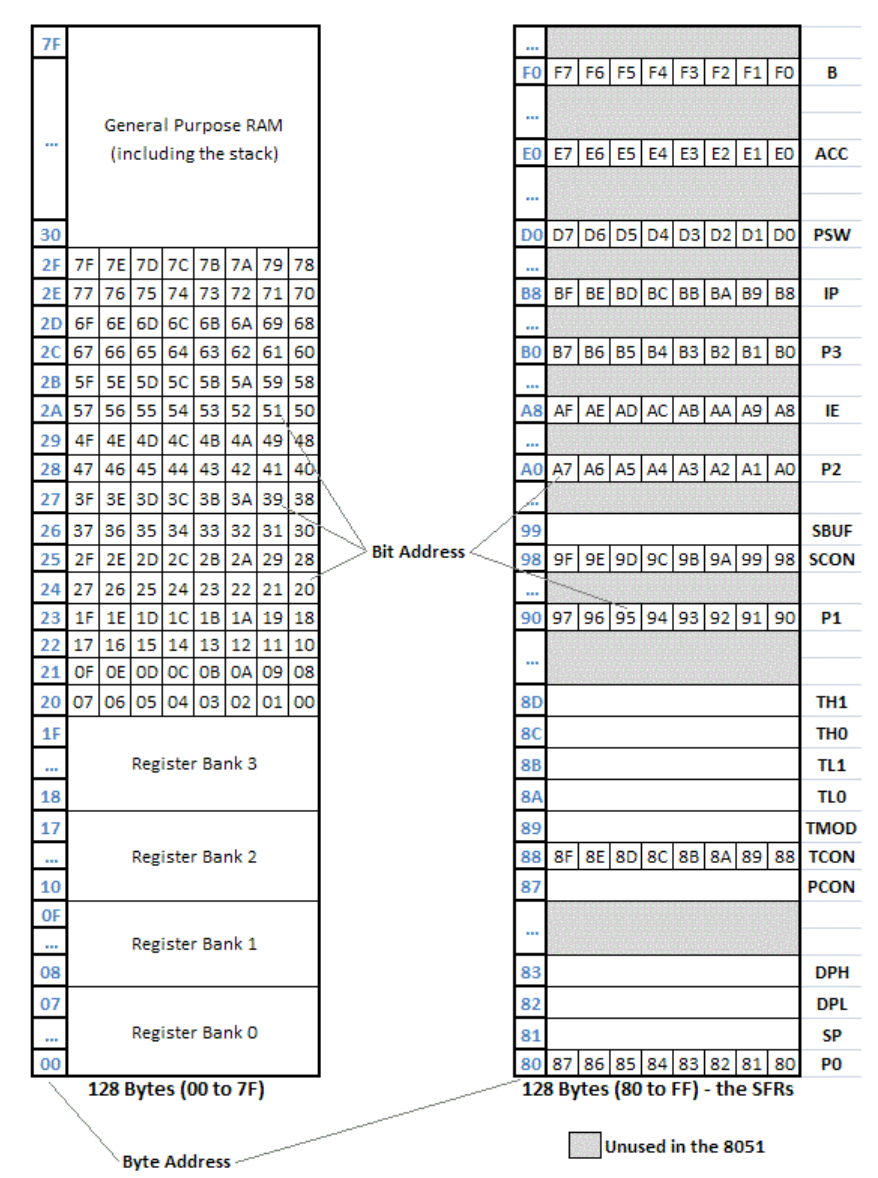
\includegraphics{img/mem.png}
}

\subsection{Program Flow}
\resizebox{3.5in}{!}{
	\begin{tabular}{c r|l}
		& 1 & program \& data read in and stored in main memory \\
		\hline
		\multirow{2}{*}{Instruction Fetch Cycle}
		& 2 & Instruction fetched from main memory \\
		& 3 & Fetched instruction is decoded and investigated \\
		\hline
		\multirow{2}{*}{Instruction Execution Cycle}
		& 4 & Operand(s) fetched \\
		& 5 & Operation performed \\
		\hline
		& 6 & GOTO 1 \\
	\end{tabular}
} %end resizebox

\subsection{Addressing Modes}
\resizebox{3.5in}{!}{
	\begin{tabular}{r|l}
		Implied Mode & operands are specified implicitly \\
		Immediate Mode & operands evaluate to values \\
		Index Mode & effective address determined by both the contents of the index register and a displacement \\
		Register Mode & operand is a register containing wanted value \\
		Direct Mode & operands are addresses pointing to wanted value \\
		Indirect Register Mode & operand is either R0 or R1, which contains an address pointing to wanted value \\
	\end{tabular}
} %end resizebox


\section{I/O}
\subsection{Pinout}
\resizebox{3.5in}{!}{
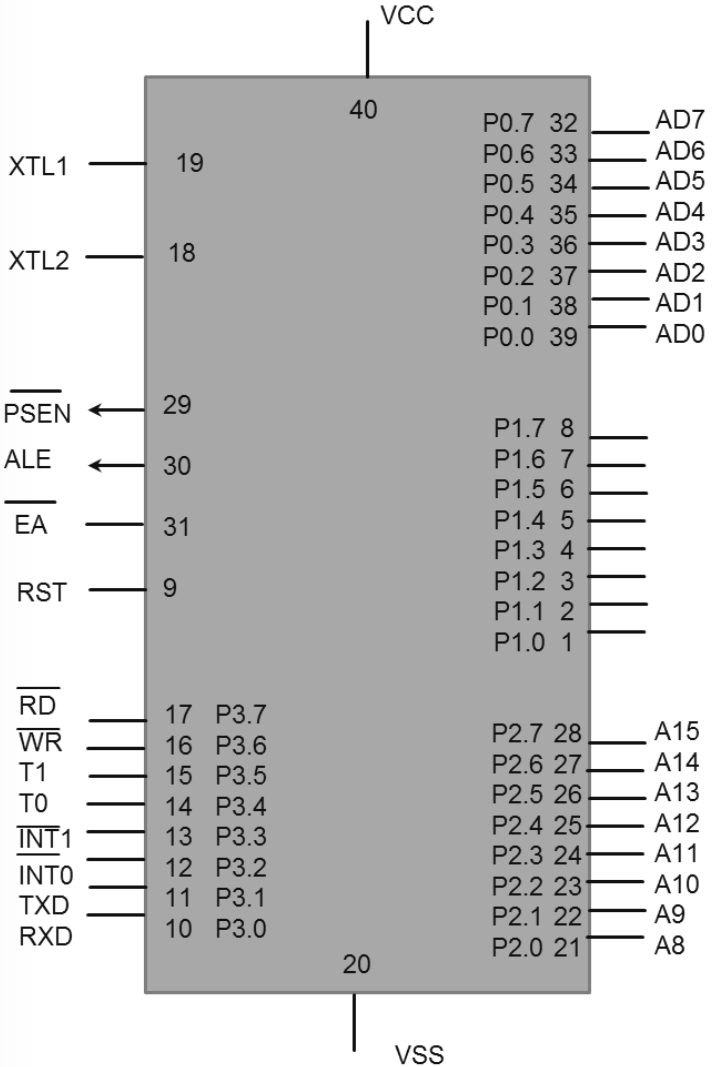
\includegraphics{img/pinout.png}
}

\subsection{Serial Port Operation}
\subsection{Timer Operation}

\pagebreak
\section{Examples}
} %end tiny
\end{document}
